\documentclass{article}
\usepackage[T1]{fontenc}
\usepackage[utf8]{inputenc}
\usepackage[polish]{babel}
\usepackage{hyperref}
\usepackage{amsmath} 
\usepackage{float}
\usepackage{graphicx}
\usepackage{siunitx}




\title{Dokumentacja projektu: Inteligentna donica}
\author{
  Julia Dobroszek 251504 \\
  Aleksander Kaźmierczak 251544 (kierownik grupy)\\
  Malwina Wodnicka 251663 \\  
}


\date{\today}

\begin{document}

\maketitle

%tabela opisujaca kto co robi
|%zrobic ladniejsza
\begin{table}[H]
    \centering
    \begin{tabular}{|c|c|}
    \hline
    członek zespołu & funkcjonalność\\
    \hline
    Olek & i2c, light, pwm, adc\\
    Malwina & gpio, audio, timer\\
    Julka & SPI, oled, czujnik temperatury\\
    \hline
    \end{tabular}
    \caption{Zawartość zespołu}
\end{table}


\section{Instrukcja użytkowania}

\subsection{Uruchomienie urządzenia}
Aby uruchomić inteligentną donicę, należy wykonać następujące kroki:
\begin{enumerate}
    \item Podłączyć urządzenie do źródła zasilania za pomocą dołączonego przewodu.
    \item Umieścić czujnik wilgotności (dwa metalowe druty) w glebie w doniczce. Czujnik powinien być umieszczony na głębokości około 3-5 cm, aby zapewnić prawidłowy pomiar wilgotności gleby.
    \item Po podłączeniu zasilania, system automatycznie rozpocznie pracę i wyświetli informacje na ekranie OLED.
    
\end{enumerate}


\subsection{Interpretacja wskaźników}
Inteligentna donica dostarcza użytkownikowi informacji o stanie rośliny poprzez:
\begin{enumerate} 
     \item \textbf{Wyświetlacz OLED} - Na ekranie prezentowane są aktualne statystyki dotyczące: 
     \begin{itemize} 
         \item Poziomu wilgotności gleby:
             \begin{itemize}
                \label{sec:wykorzystanie_ADC}
                 \item \textbf{sucho} - oznacza niski poziom wilgotności gleby (odczyt powyżej 2801), wskazujący na konieczność podlania rośliny
                 \item \textbf{w normie} - oznacza optymalny poziom wilgotności gleby (odczyt między 1601 a 2800), idealny dla wzrostu większości roślin
                 \item \textbf{mokro} - oznacza wysoki poziom wilgotności gleby (odczyt poniżej 1600), wskazujący na nadmiar wody, który może być szkodliwy dla rośliny
             \end{itemize}
         \item Temperatury otoczenia (w stopniach Celsjusza) 
         \item Natężenia światła - system interpretuje odczyt z czujnika i wyświetla jeden z trzech komunikatów:
         \begin{itemize}
             \item "jasno" - gdy wartość odczytu przekracza 2000
             \item "OK" - gdy wartość odczytu mieści się w przedziale od 350 do 2000
             \item "ciemno" - gdy wartość odczytu jest mniejsza niż 350
         \end{itemize}
         \item Dodatkowych informacji o stanie systemu 
     \end{itemize} 
     
     \item \textbf{Dioda RGB} - W zależności od poziomu wilgotności gleby, dioda RGB świeci się różnymi kolorami: 
     \begin{itemize} 
         \item Kolor żółto-zielony (\#c8ff1e) - oznacza stan \textbf{sucho} (odczyt powyżej 2801), sygnalizując potrzebę podlania rośliny
         \item Kolor zielony (\#1eff00) - oznacza stan \textbf{w normie} (odczyt między 1601 a 2800), sygnalizując optymalny poziom wilgotności
         \item Kolor błękitny (\#1effff) - oznacza stan \textbf{mokro} (odczyt poniżej 1600), sygnalizując nadmiar wody w glebie
     \end{itemize} 
 \end{enumerate}

\subsection{Kalibracja i konserwacja}
\begin{enumerate}
    \item \textbf{Kalibracja} - System został skalibrowany fabrycznie na podstawie eksperymentów empirycznych. Urządzenie nie posiada możliwości zewnętrznej kalibracji przez użytkownika.
    
    \item \textbf{Konserwacja} - Aby zapewnić prawidłowe działanie urządzenia:
    \begin{itemize}
        \item Regularnie czyścić czujnik wilgotności z osadów mineralnych, które mogą gromadzić się na jego powierzchni
        \item Utrzymywać wyświetlacz OLED w czystości, unikając bezpośredniego kontaktu z wodą
        \item Sprawdzać okresowo stan połączeń elektrycznych
        \item \textbf{Kategorycznie unikać kontaktu elektroniki z wodą} - Jedynym elementem, który może mieć bezpośredni kontakt z wilgocią, jest czujnik wilgotności (metalowe druty). Pozostałe elementy elektroniczne należy chronić przed zalaniem, zachlapaniem oraz nadmierną wilgotnością powietrza, gdyż może to prowadzić do trwałego uszkodzenia urządzenia i utraty gwarancji
    \end{itemize}
\end{enumerate}

\section{Funkcjonalności}

%olek
\subsection{Magistrala I2C}
\begin{enumerate}
    \item Interfejs I2C jest używany do komunikacji z czujnikiem światła oraz innymi komponentami wymagającymi komunikacji szeregowej. Implementacja obejmuje inicjalizację magistrali I2C, konfigurację adresów urządzeń oraz obsługę błędów komunikacji.
    \item Płytka LPC1769 posiada trzy magistrale I2C, w projekcie została użyta magistrala I2C2. 
    \item Czujnik światła jest podłączony do magistrali I2C2, a jego adres jest ustawiony na 0x44. Szczegóły konfiguracji znajdują się w sekcji \ref{sec:czujnik_swiatla}.
\end{enumerate}

\subsubsection{Omówienie rejestrów}
Rejestry mikroprocesora zostały opisane w tabeli 384. I2C register map w dokumentacji płytki. Poniżej znajdują się opisane rejestry:
\begin{itemize}
    \item \textbf{I2CONSET} - Rejestr ustawień kontrolnych I2C. Używany do ustawiania bitów w rejestrze kontrolnym I2CON. Pozwala ustawiać pojedyncze bity bez konieczności odczytywania i modyfikowania całego rejestru. Zapisanie '1' do bitu w tym rejestrze ustawia odpowiadający bit w rejestrze kontrolnym I2C. Poniżej zostały opiasne flagi:
    \begin{enumerate}
        \item Bity 0, 1 oraz 7:31 są zarezerowane 
        \item \textbf{AA} - Bit 2 \\
            Gdy:\\
            AA = 1 urządzenie wyśle ACK (czyli ustawi linię SDA w stan niski w czasie impulsu zegarowego na linii SCL). \\
            AA = 0 urządzenie wyśle NACK (czyli pozostawi linię SDA w stanie wysokim).
        \item \textbf{SI} - Bit 3 \\
            Flaga ta informuje o zmianie stanu magistrali np. zakończenie nadawania danych.
            Gdy:\\
            SI = 1, niski poziom sygnału SCL jest wydłużony. Transmisja zostaje wstrzymana.\\
            SI resetuje się poprzez zapisanie 1 do bitu SIC (SI Clear) w rejestrze I2CONCLR
        \item \textbf{STO} - Bit 4\\
            Flaga zakończenia transmisji danych. Jej działanie zależy od trybu, w jakim pracuje układ: master czy slave.\\
            W trybie master, ustawienie STO = 1 powoduje wysłanie warunku STOP na magistrali I2C, czyli SDA przechodzi z LOW na HIGH, gdy SCL jest HIGH. To kończy bieżącą transmisję i linia jest zwalniana.\\
            Gdy magistrala wykryje warunek STOP, flaga STO zostaje automatycznie wyczyszczona przez sprzęt.

        \item \textbf{STA} - Bit 5\\
            Służy do rozpoczęcia transmisji przez wysłanie warunku START
                \begin{itemize}
                    \item Jeżeli interfejs I2C jest w trybie slave, to:
                    \begin{itemize}
                        \item Interfejs przechodzi do trybu master
                        \item Jeśli magistrala jest wolna – natychmiast wysyła warunek START (SDA z HIGH do LOW przy SCL = HIGH).
                        \item Jeśli magistrala jest zajęta – czeka na warunek STOP, który „uwolni” magistralę, a potem wysyła START po pół okresie zegara wewnętrznego.
                    \end{itemize}

                    \item Jeśli interfejs już jest w trybie master, to:
                    \begin{itemize}
                        \item Ustawienie STA = 1 powoduje wysłanie repeated START – kolejnego warunku START bez wcześniejszego STOP.
                    \end{itemize}   
                    \item W przypadku, gdy STA oraz STO ustawimy jednocześnie na 1, to:
                    \begin{itemize}
                        \item w tybie master zostanie syłany sygnal STOP, następnie wysyłany jest START (restart transmisji)
                        \item w trybie slave nastąpi zatrzymanie transmisji bez wysłąnia STOP na magistralę, a następnie, jeśli magistrala jest wolna, zostanie wysłany START
                    \end{itemize}
                \end{itemize}
        \item \textbf{I2EN} - Bit 6\\
        Flaga odpowiedzialna za włączenie lub wyłączenie interfejsu I2C. Gdy:\\\
            I2EN = 0, interfejs I2C jest wyłączony\\
            I2EN = 1, interfejs I2C jest włączony
            
        
    \end{enumerate}
    \item \textbf{I2CONCLR} - Rejestr kasowania ustawień kontrolnych. Używany do kasowania bitów w rejestrze kontrolnym I2C. Zapisanie '1' do bitu w tym rejestrze kasuje odpowiadający bit w rejestrze kontrolnym I2C.
    \begin{enumerate}
        \item Bity 0, 1, 4 oraz 7:31 są zarezerowane
        \item \textbf{AAC} - Bit 2 - służy do wyzerowania bitu AA (Assert Acknowledge) w rejestrze I2CON. Bit AA odpowiada za to, czy urządzenie I2C nada ACK (potwierdzenie) podczas komunikacji.
        \item \textbf{SIC} - Bit 3 - służy do czyszczenia flagi przerwania I2C (Interrupt Clear). 
        \item \textbf{STAC} - Bit 5 - służy do czyszczenia flagi START (STA)
        \item \textbf{I2CENC} - Bit 6 - wyłącza interfejs I2C
    \end{enumerate}
    
    \item \textbf{I2STAT} - Rejestr statusu I2C. Dostarcza szczegółowe kody statusu pokazujące aktualny stan interfejsu. Z tego rejestru można tylko odczytywać dane.
    \begin{enumerate}
        \item Bity 0:2 oraz 8:31 są zarezerowane
        \item Bity 7:3 - zawierają kod aktualnego stanu interfejsu I2C.
            Kod statusu możemy wyodrębnić dzięki masce 0xF8:\\
            \begin{verbatim}
                uint8_t status = I2STAT & 0xF8;
            \end{verbatim}

            %dodac referencje do dokuemntacji lcp
            W rejestrze może wystąpić 26 kodów statusu. Kody, które mogą wystąpić znajdują się w dokumentacji LPC1769, w tabelach 399 oraz 402.\\
            Jeśli jakikolwiek z powyższych kodów wystąpi, to oznacza, że na pewno bit SI zostanie ustawiony na 1.
    \end{enumerate}
    
    
    \item \textbf{I2DAT} - Rejestr danych. Podczas trybu nadawania lub odbioru, dane (8 bitów) są zapisywane lub odczytywane z tego rejestru.   
    
    
    
    \item \textbf{I2SCLH} - Rejestr cyklu zegara SCL (wysoka połowa).Zawiera wysoką połowę cyklu zegara I2C.
    \item \textbf{I2SCLL} - Rejestr cyklu zegara SCL (niska połowa). Zawiera niską połowę cyklu zegara I2C.
    \item \textbf{MMCTRL} - Rejestr kontrolny trybu monitorowania. Używany do kontrolowania trybu monitorowania I2C.
    \item \textbf{I2DATA\_BUFFER} - Rejestr bufora danych I2C (Adres: 0x2C). Zawiera zawartość 8 najstarszych bitów rejestru przesuwnego I2DAT.
    
    \item \textbf{I2ADR0, I2ADR1, I2ADR2, I2ADR3} - Rejestry adresowe I2C. Zawierają 7-bitowy adres slave do działania interfejsu I2C w trybie slave. W na bicie 0 można ustawić czy urządzenie ma odpowiadać na GC (General Call) lub tylko na określony adres.
    \item \textbf{I2MASK0, I2MASK1, I2MASK2, I2MASK3} - Rejestry maski I2C. Służą do określenia dopasowania adresu w trybie slave.
\end{itemize}

\subsubsection{Inicjalizacja magistrali I2C2}
Inicjalizacja magistrali I2C2 odbywa się poprzez wykonanie następujących kroków:
\begin{enumerate}
    %opis ustawien konkretnych rejestrow w projekcie, uzasadnienie czemu wybralismy takie ustawienia
    \item Ustawienie odpowiednich pinów\\
        Użyte zostały piny P0.10 i P0.11, które odpowiadają pinom SCL i SDA na magistrali I2C2.\\
        Dla powyższych pinów wybrane zostały funkcje nr. 2, ponieważ z dokumentacji LPC1769 wynika, że funkcja nr. 2 odpowiada pinom SCL i SDA.\\ %odwolanie do tabeli w dokumentacji
    \item Włączenie zasilania magistrali I2C2\\
        % tabela Table 46. 
        Z tabeli 46. w dokumentacji LPC1769 można odczytać, że bit 6 w rejestrze PCONP odpowiada za włączenie zasilania magistrali I2C2.
        \[
            PCONP |= (1<<26)
        \]
    \item Ustawienie taktowania zegara\\
        Taktowanie zegara dla magistrali I2C2 ustawiamy poprzez wpisanie do rejestru I2SCLH i I2SCLL odpowiednich wartości. Wpierw pobieramy zawartość rejestru PCLK; robimy to poprzez odczytanie danych z bitów 21:20 z adresu 0x400F C1AC przy użyciu maski. Stąd wiemy, że dzielnikiem zegara jest 2, więc 
        \begin{align*}
        PCLK_{I2C2} &= \frac{CCLK}{2}\\
        I2SCLH &= \frac{PCLK_{I2C2}}{2 \cdot target\_clock}\\
        I2SCLL &= \frac{PCLK_{I2C2}}{target\_clock} - I2SCLH
        \end{align*}
            

        CCLK wynosi 100MHz. Mając powyższe wartości możemy wyliczyć taktowanie z poniższego wzoru:
        \[
        I2C_{bitfrequency} = \frac{PCLK}{I2SCLH + I2SCLL}
        \]
        Z Tabeli 395 w dokumentacji LPC1769 można odczytać, że standardowe taktowanie wynosi 100kHz, więc do rejestrów I2SCLH oraz I2SCLL wpisujemy 250
    \item Wyzerowanie flag rejestru I2CON\\
        W celu resetowania flag AC, STA, I2EN ustawiamy w rejestrze I2CONCLR bity 2, 5,6, które zerują te flagi w rejestrze I2CON.
        
    \item Włączenie magistrali I2C\\
        W celu włączenia magistrali I2C ustawiamy bit 6 w rejestrze I2CON.
\end{enumerate}

\subsubsection{Wykorzystanie magistrali I2C2}
\begin{enumerate}
    \item Początkowe ustawienia\\
        Rozpoczęcie transmisji odbywa się poprzez ustawienie flagi START w rejestraze I2CON (bit 5) na 1 oraz flagi SI (przerwanie) w rejestrze I2CON (5 bit) na 0. Później master czeka na zmianę flagi SI na 1, która oznacza, że transmisja została rozpoczęta. Następnie sprawdzany jest rejest stanu I2STAT, aby sprawdzić, czy warunek START został wysłany (0x08). Ustawiamy SI na 0.
    \item Wysyłanie danych\\
    \begin{enumerate}
        \item Wysyłanie adresu urządzenia. Adres urządzenia jest 7-bitowy. W rejestrze I2DAT należy wpisać adres urządzenia, a następnie ustawić pierwszy bit na 0, aby wskazać, że wysyłamy adres. Następnie ustawiamy flagę SI w rejestrze I2CON na 0.
        \item Master oczekuje na potwierdzenie (ACK) od slave - (z Tabeli 400) w rejestrze I2STAT powinna znajdowaćsię wartość 0x18. Gdy znajduje się tam inna wartość, to adres jest ponownie wysyłany.
        \item Po otrzymaniu ACK, master ustawia bit 5 w rejestrze I2CON (STA) na 0.
        \item Następnie master wysyła dane. W rejestrze I2DAT należy wpisać dane, które chcemy wysłać. Następnie ustawiamy flagę SI w rejestrze I2CON na 0.
        \item Oczekiwanie na ustawienie SI rejestru I2CON na 1
        \item Master oczekuje na potwierdzenie (ACK) od slave w rejestrze I2STAT powinna znajdowaćsię wartość 0x28. Gdy otrzymano ACK, to przechodzi do wysłania kolejnych danych.
    \end{enumerate}
    
    \item Odbieranie danych\\
    \begin{enumerate}
        \item Żeby wskazać adres urządzenia z któego będziemy odbierać dane należy wpisać 7-bitowy adres slave do rejestru I2DAT. Ponadto należy ustawić pierwszy bit na 1, aby wskazać, że odbieramy dane. Następnie ustawiamy flagę SI w rejestrze I2CON na 0.
        \item Master oczekuje na potwierdzenei (ACK) od slave - (z Tabeli 400) w rejestrze I2STAT powinna znajdowaćsię wartość 0x40. Gdy znajduje się tam inna wartość, to adres jest ponownie wysyłany.
        \item Po otrzymaniu ACK, master ustawia bit 5 w rejestrze I2CON (STA) na 0.
        \item Master ustawia bit 2 w rejestrze I2CON (AA) na 1, aby ustawić ACK. I odbiera bajty danych:
        \begin{enumerate}
            \item W rejestrze I2CON ustawiamy bit 3 (SI) na 0.
            \item Master czeka na zmianę flagi SI w rejestrze I2STAT
            \item Odczyt danych z I2DAT (8 bitów)
            \item przed ostatnim bajtem danych master ustawia bit 2 w rejestrze I2CON (AA) na 0, aby wyłączyć ACK.
        \end{enumerate}    
    \end{enumerate}    

    \label{sec:I2C_wysylanie_rejestrow}
    \item Zmiana i odczyt rejestrów urządzeń slave\\
    \begin{enumerate}
        \item Wysyłamy adres rejestru, który chcemy odczytać lub zmodyfikować.
        \item Jeśli chcemy modyfikować rejestr, należy wysłać nową wartość rejewstru.
        \item Jeśli chcemy odczytać, należy zacząć odbierać dane
        
    \end{enumerate}

    \item Koniec transmisji\\
    \begin{enumerate}
        \item W celu zakończenia transmisji należy ustawić bit 4 (STO) w rejestrze I2CON na 1.
        \item Zmiana wartości flagi SI w rejestrze I2CON na 0.
    \end{enumerate}


\end{enumerate}

%Malwina
\subsection{Sterowanie GPIO}

\subsubsection{Wstęp}
System wykorzystuje piny GPIO mikrokontrolera do sterowania różnymi elementami wykonawczymi donicy. Funkcjonalność ta obejmuje konfigurację kierunku pinów (wejście/wyjście), ustawianie stanów logicznych oraz obsługę przerwań sprzętowych. GPIO jest wykorzystywane między innymi do sterowania diodami sygnalizacyjnymi.

\subsubsection{Konfiguracja portów GPIO}

W systemie opartym o mikrokontroler LPC1768/9, obsługa pinów GPIO odbywa się dwuetapowo: najpierw należy przypisać pinowi odpowiednią funkcję, a następnie ustawić jego kierunek oraz zarządzać stanem logicznym.

\paragraph{Funkcja pinu}

Piny mikrokontrolera mogą pełnić różne role – od ogólnych wejść/wyjść (GPIO), przez interfejsy komunikacyjne (SPI, UART), aż po funkcje specjalne. Wybór funkcji dokonywany jest za pomocą rejestrów \texttt{PINSEL0} do \texttt{PINSEL9}, z których każdy kontroluje dwa bity odpowiadające konkretnemu pinowi:

\begin{itemize}
    \item \texttt{00} – GPIO (funkcja domyślna),
    \item \texttt{01}, \texttt{10}, \texttt{11} – funkcje alternatywne (specyficzne dla każdego pinu).
\end{itemize}

Pełna lista funkcji alternatywnych znajduje się w dokumentacji mikrokontrolera (sekcja 8.5.1 dokumentu UM10360).

\paragraph{Rejestry GPIO}

Po przypisaniu pinu funkcji GPIO, konfiguracja odbywa się za pomocą zestawu rejestrów \texttt{FIOx}, gdzie \texttt{x} oznacza numer portu (od 0 do 4). Poniżej opis poszczególnych rejestrów:

\begin{itemize}
    \item \textbf{\texttt{FIOxDIR}} – \textit{Direction Register} (Rejestr kierunku):

    Ten rejestr pozwala ustalić kierunek działania każdego pinu portu. 
    \texttt{1} ustawia dany pin jako wyjście (output), natomiast \texttt{0} oznacza wejście (input). 


    \item \textbf{\texttt{FIOxMASK}} – \textit{Mask Register} (Rejestr maski):

    Maskowanie pozwala ignorować niektóre bity przy operacjach odczytu/zapisu. 
    Bity ustawione na \texttt{1} są pomijane przez funkcje korzystające z \texttt{FIOxSET}, \texttt{FIOxCLR} i \texttt{FIOxPIN}. 
    Ustawienie bitu na \texttt{0} oznacza, że operacje na danym pinie są aktywne.


    \item \textbf{\texttt{FIOxPIN}} – \textit{Pin Value Register} (Rejestr stanu pinów):

    Ten rejestr służy zarówno do odczytu, jak i zapisu. 
    Odczyt zwraca aktualny stan logiczny wszystkich pinów danego portu, natomiast zapis nadpisuje piny wyjściowe wartościami logicznymi (jeśli są skonfigurowane jako output).


    \item \textbf{\texttt{FIOxSET}} – \textit{Set Register} (Rejestr ustawień):

    Rejestr służy do ustawiania wybranych pinów wyjściowych na stan wysoki (\texttt{logic 1}). 
    Każdy bit ustawiony na \texttt{1} wymusza stan wysoki na odpowiadającym mu pinie. 
    Ustawienie bitu na \texttt{0} nie zmienia niczego. Nie działa na pinach wejściowych.


    \item \textbf{\texttt{FIOxCLR}} – \textit{Clear Register} (Rejestr zerowania):

    Rejestr ten jest odwrotnością \texttt{FIOxSET}. Pozwala ustawić konkretne piny wyjściowe na stan niski (\texttt{logic 0}). 
    Podobnie jak wcześniej, ustawienie \texttt{1} na wybranym bicie spowoduje wyczyszczenie (ustawienie stanu niskiego) danego pinu. 
    Nie wpływa na piny wejściowe.

\end{itemize}

\subsubsection{Do czego używamy GPIO?}



\begin{table}[H]
\centering
\caption{Przypisanie pinów mikrokontrolera LPC1768/9 do obsługi układu audio LM4811}
\begin{tabular}{@{}lll@{}}
\toprule
\textbf{Pin} & \textbf{Funkcja}                  & \textbf{Opis} \\ \midrule
P0.26        & LM4811 SIGNAL                     & Generowanie sygnału dźwiękowego \\
P0.27        & LM4811 CLK                       & Sterowanie zegarem układu audio LM4811 \\
P0.28        & LM4811 UP/DN                     & Regulacja głośności LM4811 \\
P2.13        & LM4811 SHUTDOWN                  & Włączenie/wyłączenie układu LM4811 \\
\bottomrule
\end{tabular}
\end{table}

Piny są skonfigurowane jako wyjścia za pomocą funkcji GPIO i sterowane przez rejestry FIOxDIR oraz FIOxSET/FIOxCLR.


\subsubsection{Przerwania sprzętowe – opis i zastosowanie}

\begin{itemize}
    \item \textbf{Czym są przerwania sprzętowe?} \\
    Przerwania sprzętowe (ang. \textit{hardware interrupts}) pozwalają mikrokontrolerowi natychmiast reagować na określone zdarzenia zewnętrzne lub wewnętrzne, bez konieczności ich ciągłego sprawdzania w pętli głównej programu (polling).
    
    \item \textbf{Mechanizm w LPC1768/9:} \\
    Obsługa przerwań w mikrokontrolerze \textbf{LPC1768/9} opiera się na wbudowanym w rdzeń \textbf{Cortex-M3} kontrolerze \textbf{NVIC} (\textit{Nested Vectored Interrupt Controller}), który zarządza priorytetami i wywoływaniem odpowiednich procedur obsługi przerwań.
    
    \item \textbf{Typowe zastosowania przerwań:}
    \begin{itemize}
        \item zmiana stanu pinu GPIO (np. naciśnięcie przycisku),
        \item zakończenie konwersji ADC,
        \item odebranie danych przez UART, SPI czy I\textsuperscript{2}C,
        \item przepełnienie licznika lub zegara.
    \end{itemize}

    \item \textbf{Podejście w aktualnym projekcie:}
    \begin{itemize}
        \item W obecnej implementacji programu \textbf{nie są wykorzystywane przerwania}.
        \item Wszystkie operacje (odczyty czujników, sterowanie wyjściami, reakcje na zmiany warunków) są realizowane sekwencyjnie w \textbf{pętli głównej} z użyciem metody \textit{polling}.
    \end{itemize}

    \item \textbf{Zalety i ograniczenia tego podejścia:}
    \begin{itemize}
        \item \textbf{Zalety:} prostsza implementacja – brak konieczności definiowania procedur ISR (Interrupt Service Routine).
        \item \textbf{Ograniczenia:}
        \begin{itemize}
            \item mniejsze wykorzystanie potencjału mikrokontrolera,
            \item możliwe opóźnienia w reakcji na zdarzenia,
            \item ograniczona skalowalność w bardziej złożonych aplikacjach.
        \end{itemize}
    \end{itemize}
\end{itemize}







%olek
%zaimportowanie pliku z opisem czujnika swiatla
\subsection{Czujnik światła}
\label{sec:czujnik_swiatla}
Inteligentna donica wykorzystuje czujnik światła oparty na protokole komunikacyjnym I2C. Implementacja tego elementu obejmuje trzy kluczowe funkcjonalności:
ISL29003 to zintegrowany czujnik światła z 16-bitowym przetwornikiem ADC. Wewnętrzny przetwornik ADC zapewnia 16-bitową rozdzielczość, jednocześnie odrzucając migotanie 50 Hz i 60 Hz spowodowane sztucznymi źródłami światła. Ogólne zasady działania ADC zostały przedstawione w rozdziale \ref{sec:ADC}.

\begin{enumerate}
    \item \textbf{Inicjalizacja i konfiguracja czujnika ISL29003} - Proces inicjalizacji obejmuje ustawienie adresu urządzenia na magistrali I2C, konfigurację rejestrów czujnika oraz określenie parametrów pomiaru, takich jak czułość i częstotliwość próbkowania.

    \item \textbf{Odczyt danych z czujnika} - Funkcjonalność ta odpowiada za komunikację z czujnikiem poprzez protokół I2C, wysyłanie komend odczytu do odpowiednich rejestrów oraz interpretację otrzymanych danych. Implementacja uwzględnia obsługę błędów komunikacji oraz weryfikację poprawności odczytanych wartości.

    \item \textbf{Przetwarzanie i analiza danych} - Po odczytaniu surowych danych z czujnika, system przetwarza je na użyteczne informacje o poziomie natężenia światła. Funkcjonalność ta obejmuje kalibrację, filtrowanie zakłóceń oraz konwersję wartości na jednostki zrozumiałe dla użytkownika (np. luxy).
\end{enumerate}

\subsubsection{Inicjalizacja czujnika ISL29003}
    Aby zainicjować czujnik ISL29003, należy ustawić wartość 1 na 7. bicie rejestru Command (0x00). Sposób wysyłania zawartości rejestró do urządzeń podrzędnych zostałopisany w poprzednim podrozdziale \ref{sec:I2C_wysylanie_rejestrow}.

    Wysyłanie adresu urządzenia - Wysyłanie adresu urządzenia ISL29003 na magistrali I2C. Adres urządzenia to 0x44.
    Informacje na temat rejestrów i ich wartości znajdują się w dokumentacji ISL29003, w tabeli 1.\\%odwolanie do dokumentacji

    Kolejnym etapem przygotowania czujnika do pracy jest zdefiniowanie zakresu. Stałe te będą używane do przeliczania danych wyjściowych czujnika. W naszym programie ustawiamy zakres na 3892, co oznacza skalę od 0 do 3892 lux. Aby ustawić wybrane przez nas wartości zakresu (range) należy sutawić bity 3:2 (tabela 9.) w rejestrze Control (0x01) na 0:1
%tabela 9.
    \begin{table}[H]
        \centering
        \begin{tabular}{|c|c|c|}
        \hline
        Bits 3:2 & k & RANGE (k)\\
        \hline
        0:0 & 1 & 973\\
        0:1 & 2 & 3892\\
        1:0 & 3 & 15,568\\
        1:1 & 4 & 62,272\\
        \hline
        \end{tabular}
        \caption{Zakresy skali lux}
    \end{table}
    Ustawiamy także liczbę cykli zegara na konwersację analogowo cyfrową poprzez umieszczenie wartości 0:0 na bitach 1:0 w rejestrze Command (0x00) (tabela 7.)
    \begin{table}[H]
        \centering
        \begin{tabular}{|c|c|}
        \hline
        BITS 1:0 & NUMBER OF CLOCK CYCLES\\
        \hline
        0:0 & $2^{16} = 65,536$\\
        0:1 & $2^{12} = 4,096$\\
        1:0 & $2^{8} = 256$\\
        1:1 & $2^{4} = 16$\\
        \hline
        \end{tabular}
        \caption{Liczby cykli zegara}
    \end{table}

    \subsubsection{Odczyt danych z czujnika}
    Dane z ISL29003 odczytujemy przy pomocy protokołu I2C. Dane wyjściowe przechowywane są w dchów rejestrach, ponieważ odczyt jest liczbą 16-bitową. W rejestrze o adresie 0x04 znajduje się najniższy bajt danych, a w rejestrze 0x05 najwyższy bajt. Sposób odczytywania danych został opisany w podrozdziale \ref{sec:I2C_wysylanie_rejestrow}.

    \subsubsection{Przetwarzanie i analiza danych}
    Po odczytaniu danych z czujnika, system przetwarza je na użyteczne informacje o poziomie natężenia światła. Aby uzyskać wartość w luxach, należy zastosować poniższy wzór (ten wzór obowiązuje tylko gdy mamy zewnętrzny rezystor 100k$\Omega$):\\
    \[
    E = \frac{FSR \cdot DATA}{2^{n}}
    \]
    Gdzie:\\
    E - wartość w luxach\\
    FSR - zakres skali (FSR = 3892 lux)\\
    DATA - odczytana wartość z rejestru\\
    n - liczba bitów w rejestrze (16 bitów)\\

    %wstawienie zdjęcia
    \begin{figure}[H]
        \centering
        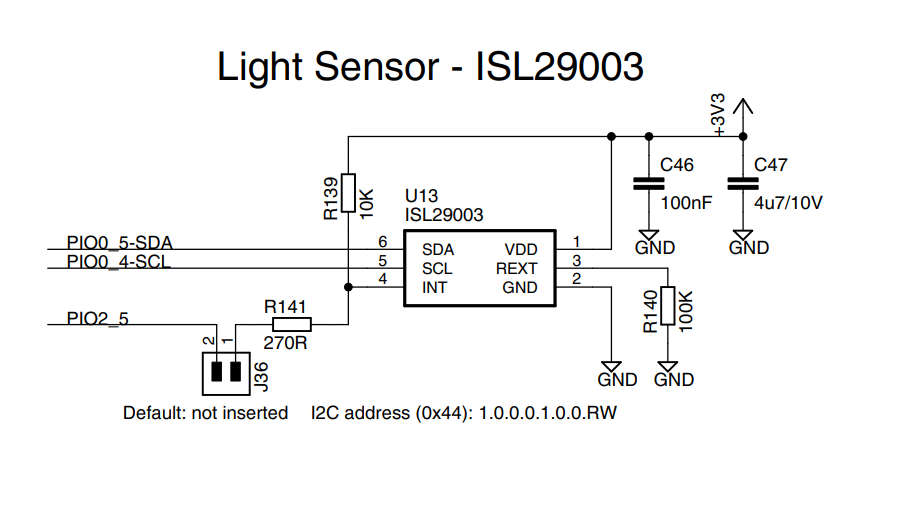
\includegraphics[width=0.8\textwidth]{../ISL29003/schemat.png}
        \caption{Schemat podłączenia czujnika ISL29003}
        \label{fig:czujnik_swiatla}
    \end{figure}


%Julka
\subsection{Czujnik temperatury}
Czujnik MAX6576 zapewnia pomiar temperatury otoczenia rośliny.

\subsubsection{Konfiguracja mikrokontrolera}

Do obsługi czujnika MAX6576 wykorzystano pin \texttt{PIO1\_5} odpowiadający pinowi \texttt{P0.2}. Konfiguracja tego pinu przebiega w następujący sposób:

\begin{itemize}
    \item \texttt{PINSEL0} – bity 5:4 ustawione na 00, konfiguracja P0.2 jako funkcję GPIO.
    \item \texttt{FIODIR0} – bit 2 ustawiony na 0, co ustawia kierunek pinu P0.2 jako wejściowy.
    \item \texttt{FIOPIN0} – odczyt wartości logicznej pinu w celu wykrywania zboczy sygnału z czujnika.
\end{itemize}

\subsubsection{Inicjalizacja i odczyt}
\begin{enumerate}
    \item Konfiguracja pinu \texttt{PIO1\_5} (P0.2) jako wejściowego.
    \item System oczekuje na zbocze sygnału wejściowego, co inicjuje pomiar czasu.
    \item Zliczanie \texttt{NUM\_HALF\_PERIODS} (tutaj 340) kolejnych zboczy sygnału z czujnika.\\
    \item Pomiar czasu \(\Delta t_{\text{ms}}\) – liczba milisekund, które upłynęły między pierwszym a ostatnim zboczem.
    \item Przeliczenie czasu na temperaturę:
    \[
    10 \cdot T(\degree \mathrm{C}) = \frac{2 \cdot 1000 \cdot \Delta t_{\text{ms}}}{\texttt{NUM\_HALF\_PERIODS} \cdot \texttt{TEMP\_SCALAR\_DIV10}} - 2731
    \]
    \begin{itemize}
        \item \(\Delta t_{\text{ms}}\) – zmierzony czas (w ms) dla zadanej liczby półokresów.
        \item \texttt{TEMP\_SCALAR\_DIV10} – współczynnik zależny od konfiguracji pinów \texttt{TS0}/\texttt{TS1} (tutaj: 1).
        \item \texttt{NUM\_HALF\_PERIODS} – liczba półokresów poddanych pomiarowi (tutaj: 340).
        \item \(2731\) – stała przeliczająca wynik z kelwinów na dziesiąte części stopnia Celsjusza.
    \end{itemize}
    \item Wykorzystanie odczytanych danych – temperatura wyświetlana jest na ekranie OLED.
\end{enumerate}



%Julka
\subsection{Magistrala SPI}
System wykorzystuje magistralę SPI z interfejsem SSP1 do komunikacji z wyświetlaczem OLED. 
Piny SPI:
\begin{itemize}
\item \textbf{P0.7} - SCK1 (Serial Clock for SSP1); generowany przez mastera sygnał zegarowy służący do synchronizacji przesyłu danych.
\item \textbf{P0.8} - MISO1 (Main In, Sub Out); służy do przesyłu danych od slave'a do mastera; SPI używamy tylko dla OLED więc MISO nie jest używany;
\item \textbf{P0.9} - MOSI1 (Main Out, Sub In); służy do przesyłu danych od mastera do slave'a;
\item \textbf{P2.2 - SSEL} (Slave Select); umożliwia wybór slave’a do transmisji, jest aktywowany stanem niskim; sterowany przez GPIO;
\end{itemize}
Rejestry magistrali SPI:
\begin{itemize}
    \item \textbf{S0SPCR} - SPI Control Register; rejestr sterujący pracą interfejsu SPI, pozwala m.in. na ustawienie trybu pracy, włączenie SPI i przerwań.
\begin{table}[H]
\centering
\caption{Opis bitów rejestru S0SPCR.}
\vspace{0.5em}
\renewcommand{\arraystretch}{1.2}
\begin{tabular}{|c|c|p{9.5cm}|}
\hline
\textbf{Bity} & \textbf{Symbol} & \textbf{Opis} \\
\hline
0–1     & —            & Zarezerwowane. \\
\hline
2       &BitEnable  & 0 – transmisja zawsze 8-bitowa, 1 – długość słowa określona przez bity 11:8 (\texttt{BITS}). \\
\hline
3       &CPHA     & Faza zegara: 0 – dane próbkowane na pierwszym zboczu, 1 – na drugim zboczu. \\
\hline
4       & CPOL       & Polaryzacja zegara: 0 – SCK aktywny wysoki, 1 – SCK aktywny niski. \\
\hline
5       & MSTR       & Tryb pracy SPI: 0 – tryb Slave, 1 – tryb Master. \\
\hline
6       & LSBF       & Kolejność bitów: 0 – MSB pierwszy, 1 – LSB pierwszy. \\
\hline
7       & SPIE       & Przerwania SPI: 0 – wyłączone, 1 – włączone (na zdarzenia SPIF lub MODF). \\
\hline
8–11    & BITS       & Liczba bitów przesyłanych w jednym transferze (aktywny tylko gdy BitEnable = 1). Patrz tabela poniżej. \\
\hline
12–31   & —            & Zarezerwowane. \\
\hline
\end{tabular}

\vspace{1em}

\begin{tabular}{|c|c|c|c|c|c|c|c|c|}
\hline
1000 & 1001 & 1010 & 1011 & 1100 & 1101 & 1110 & 1111 & 0000\\
\hline
8    & 9    & 10   & 11   & 12   & 13   & 14   & 15 & 16\\
\hline
\end{tabular}
\end{table}

    \item \textbf{S0SPSR} - SPI Status Register; rejestr stanu, zawiera flagi informujące o gotowości transmisji, zakończeniu przesyłu i błędach.

\begin{table}[H]
\centering
\caption{Opis bitów rejestru S0SPSR.}
\vspace{0.5em}
\renewcommand{\arraystretch}{1.2}
\begin{tabular}{|c|c|p{9.5cm}|}
\hline
\textbf{Bity} & \textbf{Symbol} & \textbf{Opis} \\
\hline
0–2     & —        & Zarezerwowane.\\
\hline
3       & ABRT     & Przerwanie transmisji w trybie Slave: 1 – wystąpiło przerwanie; bit czyszczony przez odczytanie tego rejestru. \\
\hline
4       & MODF     & Błąd trybu: 1 – wystąpił błąd trybu. Bit czyszczony przez odczytanie tego rejestru i zapis do rejestru kontrolnego SPI. \\
\hline
5       & ROVR     & Nadpisanie przy odczycie: 1 – wystąpił błąd przepełnienia przy odbiorze. Bit czyszczony przez odczytanie tego rejestru. \\
\hline
6       & WCOL     & Kolizja zapisu: 1 – wystąpiła kolizja przy zapisie. Bit czyszczony przez odczytanie tego rejestru i dostęp do rejestru danych SPI. \\
\hline
7       & SPIF     & Flaga zakończenia transmisji SPI: 1 – zakończono transmisję. Dla Mastera: ustawiana na końcu ostatniego cyklu; dla Slave’a: przy ostatnim zboczu próbkującym SCK. Bit czyszczony przez odczytanie tego rejestru i dostęp do rejestru danych SPI. \\
\hline
8–31    & —        & Zarezerwowane.\\
\hline
\end{tabular}
\end{table}

    
    \item \textbf{S0SPDR} - SPI Data Register; dwukierunkowy rejestr danych, zapis do niego inicjuje transmisję, odczyt zwraca dane odebrane przez SPI.

\begin{table}[H]
\centering
\caption{Opis bitów rejestru S0SPDR.}
\vspace{0.5em}
\renewcommand{\arraystretch}{1.2}
\begin{tabular}{|c|c|p{9.5cm}|}
\hline
\textbf{Bity} & \textbf{Symbol} & \textbf{Opis} \\
\hline
0-7     & DataLow  & Dwukierunkowy port danych SPI. Służy do odczytu danych odebranych lub zapisu danych do wysłania. \newline Wartość domyślna: \texttt{0x00}. \\
\hline
8–15    & DataHigh & Dodatkowe bity transmisji/odbioru, gdy bit 2 rejestru \texttt{SPCR} (BitEnable) = 1 i bity 11:8 \texttt{SPCR} są różne od \texttt{1000} (czyli liczba bitów > 8). \newline Gdy liczba bitów < 16, bardziej znaczące bity przy odczycie mają wartość zero. \newline Wartość domyślna: \texttt{0x00}. \\
\hline
16–31   & —         & Zarezerwowane. \\
\hline
\end{tabular}
\end{table}

    
    \item \textbf{S0SPCCR} - SPI Clock Counter Register; ustala częstotliwość zegara SPI (SCK) poprzez wartość dzielnika.

\begin{table}[H]
\centering
\caption{Opis bitów rejestru S0SPCCR.}
\vspace{0.5em}
\renewcommand{\arraystretch}{1.2}
\begin{tabular}{|c|c|p{9.5cm}|}
\hline
\textbf{Bity} & \textbf{Symbol} & \textbf{Opis} \\
\hline
0–7     & Counter    & Ustawienie licznika zegara SPI0. \newline Wartość musi być parzysta i większa lub równa 8. Określa częstotliwość zegara SPI:  
\[ \text{SCK}_{\text{freq}} = \frac{PCLK}{\text{Counter}} \]
\newline Wartość domyślna: \texttt{0x00}. \\
\hline
8–31    & —          & Zarezerwowane.\\
\hline
\end{tabular}
\end{table}

    
    \item \textbf{S0SPINT} - SPI Interrupt Flag; flaga informująca o wystąpieniu przerwania SPI; może być programowo wyczyszczona.

    \begin{table}[H]
\centering
\caption{Opis bitów rejestru S0SPINT}
\vspace{0.5em}
\renewcommand{\arraystretch}{1.2}
\begin{tabular}{|c|c|p{9.5cm}|}
\hline
\textbf{Bity} & \textbf{Symbol} & \textbf{Opis} \\
\hline
0     & SPIF       & Flaga przerwania SPI. Ustawiana przez interfejs SPI w celu wygenerowania przerwania. \newline Zerowana przez zapisanie jedynki do tego bitu. \newline \\
\hline
1–7   & —          & Zarezerwowane.\\
\hline
8–31  & —          & Zarezerwowane. \\
\hline
\end{tabular}
\end{table}
\end{itemize}
Rejestry SSP:
\begin{itemize}
  \item \textbf{CR0} – Control Register 0; ustala rozmiar słowa danych, tryb protokołu SPI oraz współczynnik dzielnika zegara.
  \item \textbf{CR1} – Control Register 1; konfiguruje tryb master/slave i inne ustawienia pracy kontrolera SSP.
  \item \textbf{DR} – Data Register; rejestr danych – zapis wypełnia FIFO nadawcze, odczyt opróżnia FIFO odbiorcze.
  \item \textbf{SR} – Status Register; rejestr stanu – zawiera flagi informujące o stanie transmisji i buforów FIFO.
  \item \textbf{CPSR} – Clock Prescale Register; dzielnik preskalera zegara – ustala podstawową częstotliwość SSP.
  \item \textbf{IMSC} – Interrupt Mask Set and Clear Register; umożliwia maskowanie (włączanie/wyłączanie) poszczególnych źródeł przerwań.
  \item \textbf{RIS} – Raw Interrupt Status Register; pokazuje status aktywnych przerwań niezależnie od ustawienia masek.
  \item \textbf{MIS} – Masked Interrupt Status Register; pokazuje status przerwań uwzględniający ustawienia masek.
  \item \textbf{ICR} – Interrupt Clear Register (SSPICR); służy do ręcznego kasowania wybranych flag przerwań.
  \item \textbf{DMACR} – DMA Control Register; umożliwia włączenie transmisji danych za pomocą kontrolera DMA.
\end{itemize}


%Julka
\subsection{Wyświetlacz OLED}

Wyświetlacz OLED model UG-9664HSWAG01 (oznaczenie na schemacie OLED1) komunikuje się przez interfejs SPI. Wyświetlacz bazuje na sterowniku SSD1305 132 x 64 Dot Matrix OLED/PLED Segment/Common Driver with Controller. Wyświetlacz służy jako interfejs użytkownika, prezentując dane w czytelnej formie graficznej.

\subsubsection{Konfiguracja}
Piny sterujące wyświetlaczem OLED:
\begin{itemize}
\item \textbf{P0.6} – CS (Chip Select); aktywny w stanie niskim;
\item \textbf{P2.7} – D/C (Data/Command); w stanie wysokim dane są traktowane jako dane, w stanie niskim przesyłane do rejestru komend.
\item \textbf{P2.1} - RES (reset); w stanie niskim wywołuje reset i inicjalizację, w trakcie normalnej pracy należy utrzymywać go w stanie wysokim;
\end{itemize}
\subsubsection {Inicjalizacja:}
\begin{enumerate}
    \item Ustawiamy piny 2.1, 2,7 oraz 0.6 w tryb wyjścia za pomocą rejestrów GPIO. %Odwołanie do GPIO rejestrów FIODIR
    \item Ustawiamy pin 2.1 w tryb niskiego stanu aby upewnić się, że wyświetlacz jest wyłączony.
    \item Wysyłamy instrukcje inicjalizujące do wyświetlacza OLED.
    \item Odczekujemy krótki czas przed włączeniem wyświetlacza.
    \item Ustawiamy pin 2.1 w tryb wysokiego stanu aby włączyć wyświetlacz.
\end{enumerate}
\subsubsection {Przesyłanie danych:}
\label{przes}
\begin{enumerate}
    \item Ustawienie pinu CS w stan niski.
    \item Ustawienie pinu D/C w stan wysoki w trybie danych lub w stan niski w trybie komendy.
    \item Przygotowanie struktury transferu.
    \item Inicjacja transmisji SPI.
    \item Ustawienie pinu CS w stan wysoki.
\end{enumerate}

\subsubsection {Rysowanie pojedynczego piksela}
\label{piksel}
\begin{enumerate}
    \item Na podstawie współrzędnej y określany jest numer strony (ang. page address) — każda strona odpowiada 8 poziomym liniom pikseli w pamięci graficznej SSD1305.
    \item Obliczany jest adres kolumny x, przy czym należy uwzględnić fakt, że kontroler SSD1305 obsługuje rozdzielczość 132x64 piksele, natomiast fizyczny wyświetlacz posiada tylko 96x64 piksele, co oznacza konieczność stosowania przesunięcia poziomego podczas adresowania kolumn.
    \item Na podstawie współrzędnej y wyliczany jest numer bitu (0–7), który odpowiada konkretnej pozycji w bajcie strony, a następnie tworzona jest odpowiednia maska bitowa.
    \item W buforze cieniowania wykonywana jest modyfikacja odpowiedniego bajtu: bit jest ustawiany lub czyszczony w zależności od wartości koloru (czarny/biały).
    \item Ustawiany jest adres w pamięci wyświetlacza (komendy: wybór strony, kolumny niskiej i wysokiej).
    \item Bajt danych z bufora cieniowania (zaktualizowany) jest przesyłany przez interfejs SPI do pamięci graficznej wyświetlacza tak jak opisano w \ref{przes}.
\end{enumerate}

\subsubsection{Wyświetlanie pojedynczego znaku}
\begin{enumerate}
    \item Z tablicy font5x7 pobierany jest odpowiedni wzorzec bitowy znaku (bitmapa o wysokości 8 linii).
    \item Dla każdej z 8 linii (wierszy) znaku:
    \begin{itemize}
        \item Wczytywany jest bajt danych określający wzorzec piksela w danym wierszu.
        \item Iteracja po 6 kolumnach piksela w danej linii:
        \begin{itemize}
            \item Jeśli odpowiedni bit w bajcie danych jest ustawiony — wybierany jest kolor pierwszoplanowy, W przeciwnym razie — kolor tła).
            \item Ustawienie danego piksela zgodnie z kolorem i współrzędnymi \ref{piksel}.
        \end{itemize}
    \end{itemize}
    \item Po przerysowaniu całej linii znakowej kursor pionowy jest przesuwany w dół o jeden piksel, a poziomy resetowany do początkowej pozycji.
\end{enumerate}

\subsubsection{Wyświetlanie ciągu znaków i wypełnienie prostokąta}

Wyświetlenie ciągu znaków i wypełnienie prostokąta realizowane są w oparciu o te same mechanizmy niskopoziomowe co rysowanie pojedynczego piksela, znaku, przy czym operacje te są zoptymalizowane pod kątem wydajności poprzez grupowanie zapisów do pamięci wyświetlacza.

W przypadku ciągów znaków każdy znak traktowany jest jako zestaw pikseli, a wypełnienie prostokąta sprowadza się do sekwencyjnego ustawiania bloków pikseli w określonym obszarze, co minimalizuje liczbę koniecznych operacji adresowania.



%Malwina
\subsection{System audio}
System audio inteligentnej donicy składa się z głośnika (oznaczenie na schemacie SP1) oraz układu sterowania LM4811MM (oznaczenie na schemacie U10). Układ ten umożliwia generowanie sygnałów dźwiękowych informujących użytkownika o stanie rośliny. Implementacja obejmuje inicjalizację układu sterowania, konfigurację parametrów dźwięku oraz bibliotekę funkcji do odtwarzania różnych melodii w zależności od poziomu wilgotności gleby.


%Malwina
\subsection{Timer}
System wykorzystuje timery sprzętowe mikrokontrolera do precyzyjnego odmierzania czasu i wykonywania cyklicznych zadań. W przeciwieństwie do PWM, który służy do generowania sygnałów o zmiennym wypełnieniu, timery są wykorzystywane do wywoływania przerwań w określonych odstępach czasu. Funkcjonalność ta obejmuje konfigurację preskalerów, rejestrów porównania oraz obsługę przerwań. Timery są używane do planowania pomiarów, kontroli cykli nawadniania oraz implementacji funkcji oszczędzania energii.

%olek
%zaimportowanie pliku z opisem pwm


\definecolor{dkgreen}{rgb}{0,0.6,0}
\definecolor{gray}{rgb}{0.5,0.5,0.5}
\definecolor{mauve}{rgb}{0.58,0,0.82}

\lstdefinestyle{customc}{
  belowcaptionskip=1\baselineskip,
  breaklines=true,
  frame=L,
  xleftmargin=\parindent,
  language=C,
  showstringspaces=false,
  basicstyle=\footnotesize\ttfamily,
  keywordstyle=\bfseries\color{green!40!black},
  commentstyle=\itshape\color{purple!40!black},
  identifierstyle=\color{blue},
  stringstyle=\color{orange},
}

\lstdefinestyle{customasm}{
  belowcaptionskip=1\baselineskip,
  frame=L,
  xleftmargin=\parindent,
  language=[x86masm]Assembler,
  basicstyle=\footnotesize\ttfamily,
  commentstyle=\itshape\color{purple!40!black},
}

\lstset{escapechar=@,style=customc}

\subsection{Modulacja szerokości impulsu (PWM)}
Implementacja PWM umożliwia precyzyjne sterowanie elementami wykonawczymi wymagającymi sygnału analogowego, takimi jak silniki czy regulacja jasności diody LED. Funkcjonalność obejmuje konfigurację częstotliwości sygnału PWM, ustawianie wypełnienia impulsu (duty cycle) oraz dynamiczną zmianę parametrów w zależności od warunków środowiskowych. PWM jest wykorzystywane do regulacji intensywności świecenia diod LED w diodzie RGB LED3 [schemat]. %dodaj schemat
W projekcie został wykorzystany PWM1.

\subsubsection{Inicjalizacja PWM1}
\begin{enumerate}
    \item Konfigurację rozpoczynamy od włączenia zasilania. W tym celu ustawiamy 6 bit w rejestrze PCONP (tabela 46.) %odwolanie do dokumentacji
    \item Piny na których chcemy sterować impulsami to P2.0, P2.1, P2.2. Chcemy je ustawić jako PWM1.1, PWM1.2, PWM1.3, dlatego w rejestrze PINSEL4 ustawiamy bity 1:0, 3:2, 5:4 na 01 - funkcja PWM1.X
    % \item Następnie wybieramy tryb pracy na single edge, czyli
    \item Opis rejestrów PWM1:\\
    \begin{enumerate}
        \item \textbf{IR} - rejestr ten służy do zarządzania przerwaniami. Przerwania 
        \begin{enumerate}
            \item \textbf{PWMMR0 Interrupt} - bit 0, flaga przerwania na kanale 0
            \item \textbf{PWMMR1 Interrupt} - bit 1, flaga przerwania na kanale 1
            \item \textbf{PWMMR2 Interrupt} - bit 2, flaga przerwania na kanale 2
            \item \textbf{PWMMR3 Interrupt} - bit 3, flaga przerwania na kanale 3
            \item \textbf{PWMCAP0 Interrupt} - bit 4, flaga przerwania dla zerowego wejscia przechwytującego (capture input); capture oznacza przechwycenie aktualnej wartości licznika (timer'a), np. w momencie zbocza sygnału (narastającego lub opadającego) na pinie wejściowym. Umożliwia to np. pomiar czasu trwania impulsów, okresów czy częstotliwości.
            \item \textbf{PWMCAP1 Interrupt} - bit 5, flaga przerwania dla pierwszego wejscia przechwytującego 
            \item Bity 7:6 - zarezerwowane
            \item \textbf{PWMMR4 Interrupt} - bit 8, flaga przerwania na kanale 4
            \item \textbf{PWMMR5 Interrupt} - bit 9, flaga przerwania na kanale 5
            \item \textbf{PWMMR6 Interrupt} - bit 10, flaga przerwania na kanale 6
            \item Bity 31:11 - zarezerwowane

        \end{enumerate}
        \item \textbf{PWM1TCR}
        \begin{enumerate}
            \item \textbf{Counter Enable} - bit 0, włączanie i wyłączanie licznika timera oraz preskalera
            \item \textbf{Counter Reset} - bit 1, resetowanie licznika timera, synchoronizacja z kolejnym zboczem narastającym PCLK, tak długo, aż wartość tego bitu będzie równa 1
            \item Bit 2 - zarezerwowany
            \item \textbf{PWM Enable} - gdy wartość bitu jest róna 1 - \textbf{tryb PWM}, licznik resetuje się do 1, aktywuje shadow registery.\\
                            Gdy wartość bitu jest równa 0 - \textbf{tryb timer}, licznik resetuje się do 0, bez PWM - działą jak zwykły timer.
            \item Bit 4:31 - zarezerwowane
        \end{enumerate}
        \item \textbf{PWM1CTCR} - rejestr służy do wyboru trybu licznika - timer lub jako licznik zliczający impulsy z zewnętrznego źródła. 
        \begin{enumerate}
            \item \textbf{Counter/Timer Mode} - bity 0:1, wartości i odpowiadające im działanie zostały opisane w poniższej tabeli.
            \begin{table}[H]
                \centering
                \begin{tabular}{|c|p{13cm}|}
                    \hline
                    \rowcolor{gray!30}
                    Wartość & Opis\\
                    \hline
                    00  & Timer mode: Timer Counter (TC) wykorzystuje Prescale Counter (PC) oraz Prescale Register (PR), aby móc działać wolniej. TC inkrementuje się gdy PC = PR\\
                    \hline
                    01 & Counter Mode: TC zlicza impulsy przychodzące (inkrementacja przy każdym zboczu narastającym) z zewnętrznego pinu wybranego na bitach 3:2  \\
                    \hline
                    10 & Counter Mode: TC zlicza impulsy przychodzące (inkrementacja przy każdym zboczu opadającym) z zewnętrznego pinu wybranego na bitach 3:2  \\
                    \hline
                    11 & Counter Mode: TC zlicza impulsy przychodzące (inkrementacja przy na obu zboczach impulsu) z zewnętrznego pinu wybranego na bitach 3:2  \\
                    \hline
                \end{tabular}
                \caption{Rodzaje pracy w trybie Timer/Counter}
            \end{table}
            \item \textbf{Count Input Select} - bity 3:2 - ta częśćrejestru odpowiada za wybó pinu PCAP z którego będą zliczane impulsy.\\
            \begin{table}[H]
                \centering
                \begin{tabular}{|c|p{13cm}|}
                    \hline
                    \rowcolor{gray!30}
                    Wartość & Opis\\
                    \hline
                    00  & Timer mode: Timer Counter (TC) wykorzystuje Prescale Counter (PC) oraz Prescale Register (PR), aby móc działać wolniej. TC inkrementuje się gdy PC = PR\\
                    \hline
                    01 & Counter Mode: TC zlicza impulsy przychodzące (inkrementacja przy każdym zboczu narastającym) z zewnętrznego pinu wybranego na bitach 3:2  \\
                    \hline
                    10 & Counter Mode: TC zlicza impulsy przychodzące (inkrementacja przy każdym zboczu opadającym) z zewnętrznego pinu wybranego na bitach 3:2  \\
                    \hline
                    11 & Counter Mode: TC zlicza impulsy przychodzące (inkrementacja przy na obu zboczach impulsu) z zewnętrznego pinu wybranego na bitach 3:2  \\
                    \hline
                \end{tabular}
                \caption{Rodzaje pracy w trybie Timer/Counter}
            \end{table}
            
            \item \textbf{PWM1MCR} - steruje reakcjami układu PWM, gdy zawartość rejestru licznika czasowego PWM Timer Counter (TC) jest równa jednej z wartości w rejestrach dopasowania PWM Match Registers (MR0–MR6). Ustawienie jedynki na poniższych bitach powoduje włączenie danej funkcji.
            \begin{enumerate}
                \item \textbf{PWMMR0I} - bit 0, gdy rejestr licznika PWM (PWM Timer Counter) osiągnie wartość ustawioną w Match Register 0 – PWMMR0, może wystąpić przerwanie - jeśli wartość ustawiona na tym bicie to 1
                \item \textbf{PWMMR0R} - bit 1, gdy zawartość licznika PWMTC jest równa wartości PWMMR0 nastąpi reset PWMTC; Pozwala to tworzyć cykliczny sygnał PWM – licznik odlicza od 0 do wartości w PWMMR0, potem reset.
                \item \textbf{PWMMR0S} - bit 3, zatrzymuje licznik, gdy wartość w rejestrze PWMTC jest równa wartości zapisanej w PWMMR0
                \item funkcjonalności kolejnych bitów tego rejestru są cyklicznie powtarzane dla PWMMR1f, PWMMR2f, PWMMR3f, PWMMR4f, PWMMR5f, PWMMR6f (gdzie 'f' oznacza numer rejestru PWMMR)\\
                                        Bity 21:31 są zarezerwowane.
            \end{enumerate}

            \item \textbf{PWM1CCR} - rejestr pozwala skonfigurować zdarzenia przechwytywania (capture events) na wejściach CAPn.x, czyli kiedy wartość licznika zostanie zapisana do rejestru przechwytywania (CRn), gdzie n jest numerem Timera - 0 lub 1. Warto zaznaczyć, że jeśli CAP input jest skonfigurowane jako źródło zliczania (Counter Mode w CTCR), to jego bity w PWM1CCR muszą mieć wartość 000.
                Poniższe funkcje są dostępne przy ustawieniu flagi na 1 we wskazanym bicie.
                \begin{enumerate}
                    \item \textbf{Capture on CAPn.0 rising edge} - bit 0, jeśli zostanie wykryte zbocze narastające, to do rejestru przechwytywania CR0 zostanie wpisana zawartość TC
                    \item \textbf{Capture on CAPn.0 falling edge} - bit 1, jeśli zostanie wykryte zbocze opadające, to do rejestru przechwytywania CR0 zostanie wpisana zawartość TC
                    \item \textbf{Interrupt on CAPn.0 event} - bit 3, jeśli zostanie wykryte zdarzenie przechwycenia, to zawartośćTC zostanie wpisana do CR0 oraz zostanie wygenerowane przewanie
                    \item Takie same funkcje mają bity 5:3, ale dla CAPn.1 i zapis do CR1.
                    \item Bity 31:6 są zarezerwowane.
                \end{enumerate}
            \item \textbf{PWM1PCR} - rejestr służy do włączania PWM oraz wybierania trybu działąnia kanału.
                \begin{enumerate}
                    \item \textbf{PWMSELx} - wybór trybu pracy dla kanału PWMx, gdzie x to numery 2-6.\\
                        Poniższa tabela opisuje generowany impuls w zależności od ustawionego bitu. \\
                        Bity 0:1 sąnieużywane, zawsze mają wartość 0.\\
                        Bity 7:8 - są zarezerwowane.\\
                        Zatem bity ustawiające tryby pracy to 6:2.
                        \begin{table}[H]
                            \centering
                            \begin{tabular}{|c|c|p{10cm}|}
                                \hline
                                \rowcolor{gray!30}
                                Wartość & Tryb & Opis\\
                                \hline
                                    0 & Single-edge & Generowany jest impuls z jedną \hyperref[fig:single-edge-left-pwm]{krawędzią opadającą}, ponieważ z \href{https://www.zsk.p.lodz.pl/~morawski/SCR&ES/NotyKatalogowe/UM10360.pdf#page=119&zoom=100,210,814}{dokumentacji (strona 520)}., wynika iż każdy cykl PWM zaczyna się od stanu wysokiego.\\
                                \hline
                                    1 & Double-edge & Generowany jest impuls z \hyperref[fig:double-edge-center-pwm]{dwiema krawędziami} (umożliwia symetryczne impulsy)\\
                                \hline
                            \end{tabular}
                            \caption{Rodzaje pracy w trybie Timer/Counter}
                        \end{table}

                        \begin{figure}[H]
                            \centering
                            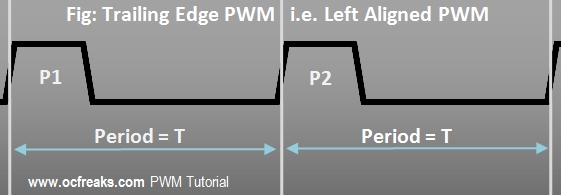
\includegraphics[width=0.8\textwidth]{../PWM/single_edge_left.jpg}
                            \caption{Przedstawienie trybu single-edge PWM, lewy impuls}
                            \label{fig:single-edge-left-pwm}
                        \end{figure}

                        \begin{figure}[H]
                            \centering
                            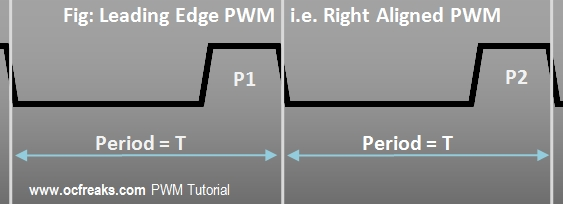
\includegraphics[width=0.8\textwidth]{../PWM/single_edge_right.jpg}
                            \caption{Przedstawienie trybu single-edge PWM, prawy impuls}
                            \label{fig:single-edge-right-pwm}
                        \end{figure}

                        \begin{figure}[H]
                            \centering
                            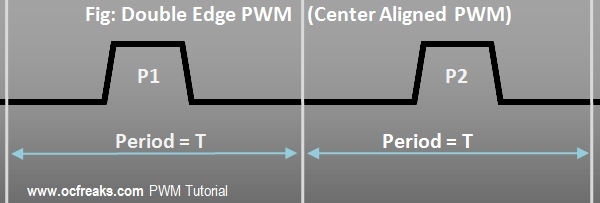
\includegraphics[width=0.8\textwidth]{../PWM/double-edge-center-pwm.jpg}
                            \caption{Przedstawienie trybu double-edge PWM}
                            \label{fig:double-edge-center-pwm}
                        \end{figure}
                    
                        \item \textbf{PWMENAx} - służy do włączania lub wyłączania wyjścia PWM, gdzie x to numer kanału PWM (1-6). Ustawianie tych funkcji odbywa się na bitach 14:9. Wartość 1 włącza wyjście, a wartość 0 wyłącza. Bity 15:31 są nieużywane i mają wartość 0.
                        \item \textbf{PWM1LER} - używany jest do aktualizacji rejestró PWM Match, ponieważ w trybie PWM Mode, wartości wpisywane do rejestrów dopasowania nie są od razu używane, ale trafiają do rejestrów tymczasowych (shadow registers). Zmiany należy zatwierdzić poprzez ustawienie odpowiednich bitó w PWM1LER. Zmiany są widoczne dopiero po rozpocząciu nowego cyklu PWM.
                        %MR0 - sufit - koniec cyklu
                        %MRx (x = 1–6) = moment zbocza opadającego
                        %W trybie single edge: zbocze narastające zawsze w 0
                        %W double edge: zbocza mogą być ustawione niezależnie w MRx i MRy (np. MR1 i MR2)
                \end{enumerate}
            
                

        \end{enumerate}

        
    \end{enumerate}

    \item Omówienie zagadnienia PWM na podstawie sterowania diodą LED3. \\
        LED3, to dioda RGB, skłądająca się z oddzielnych diod czerwonej, zielonej i niebieskiej (wspólny plus). Wykorzystanie PWM do pośredniego (sterujemy masą poprzez tranzystory \hyperref[fig:led3]{(schemat)}) sterowania jasnością diod RGB umożliwia dostosowanie jasności poszczególnych kolorów w zależności od potrzeb.
        \begin{figure}[H]
            \centering
            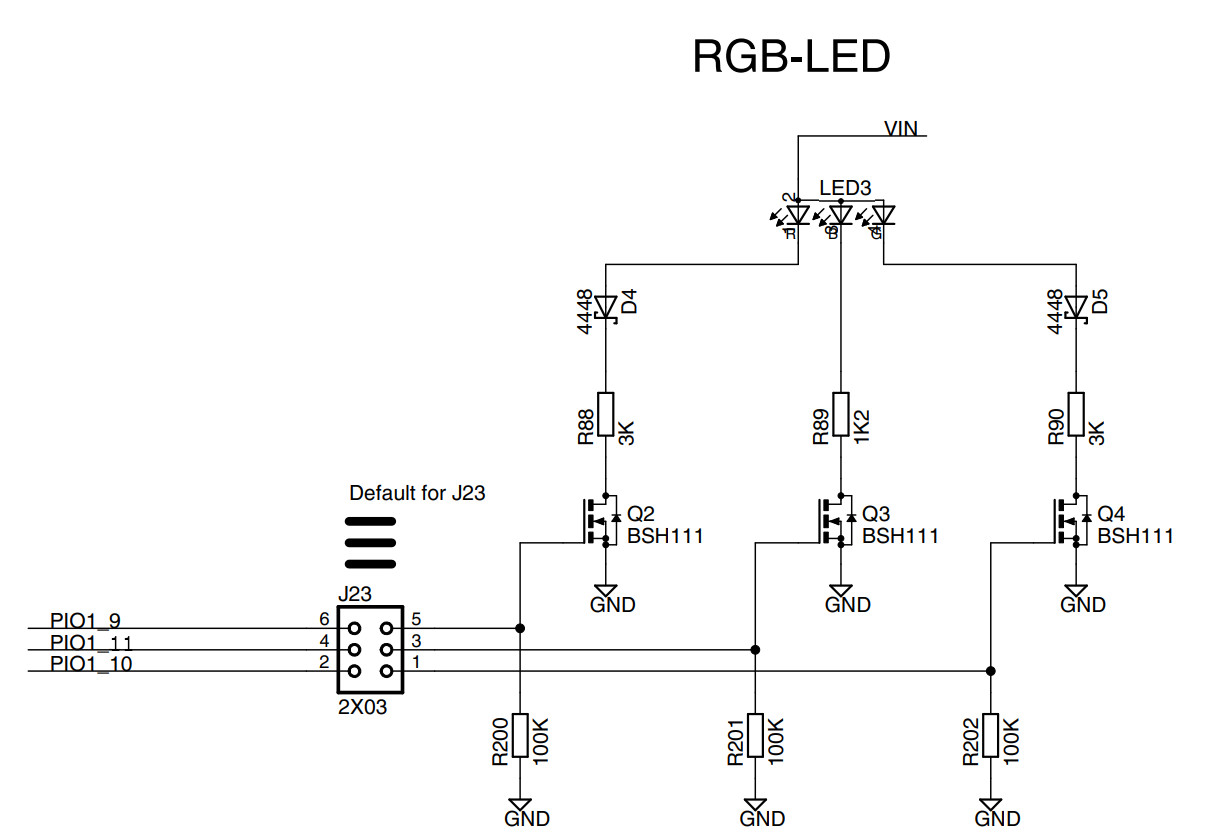
\includegraphics[width=0.8\textwidth]{../PWM/led3.jpg}
            \caption{Schemat diody RGB}
            \label{fig:led3}
        \end{figure}
        
        Jasność diody jest skorelowana z szerokością impulsu. Ze względu na zapis szestnastkowy kolorów RGB (każdy kolor ma zakres 0-255), zdecydowaliśmy się na okres 255.
        \begin{lstlisting}
LPC_PWM1->PCR = (1 << 9) | (1 << 10) | (1 << 11);  // ustawiamy tryb PWM na single-edge

LPC_PWM1->PR = 0;         // TC jest inkrementowany przy PR+1, wiec dzielnik zegara sie nie zmienia. 
                          // Czestotliwosc wynosi 25 MHz / 1 = 25 MHz
LPC_PWM1->MR0 = 255;      // Okres PWM = 255 cykli 
LPC_PWM1->MCR = (1 << 1); // Reset na MR0 (PWM cycle)

LPC_PWM1->MR1 = 255;      // Ustawiamy jasnosc na 100%, szerokosc impulsow = 255 / 255 = 100%
LPC_PWM1->MR2 = 255;      
LPC_PWM1->MR3 = 255; 

LPC_PWM1->LER = (1 << 1) | (1 << 2) | (1 << 3) | (1 << 0); // Aktualizacja rejestrow MRx

LPC_PWM1->TCR = (1 << 0) | (1 << 3);  // Wlaczamy PWM
        \end{lstlisting}

        Kolor LED3 ustawiamy przy pomocy funkcji $PWM_SetColor(uint8_t red, uint8_t green, uint8_t blue)$, która zmienia zawartość rejestrów MR1, MR2 i MR3.
        
        \begin{lstlisting}
void PWM_SetColor(uint8_t red, uint8_t green, uint8_t blue) {
    if( red < 0 || red > 255 ) return; // ograniczenie zakresu
    if( green < 0 || green > 255 ) return;
    if( blue < 0 || red > 255 ) return;

    LPC_PWM1->MR1 = red; // ustawiamy szerokosc impulsu dla diody czerwonej
    LPC_PWM1->MR2 = blue; // ustawiamy szerokosc impulsu dla diody niebieskiej
    LPC_PWM1->MR3 = green; // ustawiamy szerokosc impulsu dla diody zielonej

    LPC_PWM1->LER = (1 << 1) | (1 << 2) | (1 << 3);  // zaktualizuj MR1-MR3
}
        \end{lstlisting}
\end{enumerate}








%olek

\subsection{Przetwornik analogowo-cyfrowy (ADC)}
\label{sec:ADC}
System wykorzystuje przetwornik analogowo-cyfrowy do odczytu analogowego wejścia czujnika określanego jako "czujnik wilgotności". Należy zaznaczyć, że termin "wilgotność" jest w tym przypadku skrótem myślowym, ponieważ w rzeczywistości nie mierzymy bezpośrednio wilgotności gleby, a jej przewodność elektryczną, która jest skorelowana z zawartością wody w glebie. Implementacja obejmuje:
Wbudowany przetwornik ADC jest przetwornikiem 12-bitowym, co oznacza, że może zwracać wartość z zakresu 0-4095. Przetwornik ten działa przy użyciu metody SAR (Successive Approximation Register), która polega na sekwencyjnym przybliżaniu wartości.
\begin{enumerate}
    \item \textbf{Inicjalizacja i konfiguracja przetwornika ADC} - Proces inicjalizacji obejmuje konfigurację rejestrów mikrokontrolera, ustawienie częstotliwości próbkowania, wybór kanału pomiarowego oraz określenie napięcia referencyjnego. ADC może wykonać do 200 000 konwersji na sekundę (200 kHz), przy pełnej 12-bitowej rozdzielczości. To znaczy, że maksymalnie co 5 mikrosekund może być gotowy nowy wynik pomiaru. 
    
    \item \textbf{Odczyt wartości analogowej} - Funkcjonalność ta odpowiada za uruchomienie konwersji analogowo-cyfrowej, odczyt wyniku konwersji oraz obsługę ewentualnych błędów pomiaru.
    
    \item \textbf{Interpretacja danych pomiarowych} - System przetwarza odczytane wartości na względny poziom wilgotności gleby. Proces ten obejmuje kalibrację czujnika (określenie wartości dla suchej i mokrej gleby), filtrowanie zakłóceń oraz konwersję surowych danych na format zrozumiały dla użytkownika.
\end{enumerate}


%chapter 29.
\subsubsection{Inicjalizacja przetwornika ADC}
    \begin{enumerate}
        \item Na początku ustawiono piny do pracy w trybie analogowym. Dla pinu 23 na porcie 0 ustawiono funkcję nr. 1, co jest odpowiednikiem funkcji analogowej (Tabela 81.) \\%odwolanie do dokumentacji
              Aby ustawić wybraną funkcję, należy ustawić bity 15:14 w rejestrze PINSEL1 na 01.
        \item Następnie ustawiono 12. bit w rejestrze PCONP o adresie 0x400F C0C4 na 1, aby włączyć zasilanie dla przetwornika ADC.
        \item Kolejniym krokiem jest odczytanie dzielnika zapisanego w rejestrze PCLKSEL0 o adresie 0x400F C1A8 na bitach 25:24 (Tabela 40.). Domyślnie dzielnik ten wynosi 4 (w rejestrze pod podanymi bitami znajduje się 00). Wtedy obowiązuje wzór na PCLK:
        
        \begin{equation*}
            PCLK = \frac{CCLK}{4}
        \end{equation*}
            
        Gdzie:
        \begin{align*}
        \text{CCLK} & - \text{takt zegara układu};\quad CCLK = 100\,\text{MHz} \\
        \text{PCLK} & - \text{takt zegara przetwornika ADC}
        \end{align*}
    \end{enumerate}

\subsubsection{Obliczanie masek do odczytu wartości rejestrów}
        Aby móc zmieniać stan przetwarzania potrzebna jest maska, która pozwoli wybrać tylko interesujące nas bity z rejestru AD0CR.
        \begin{enumerate}
            \item W rejestrze AD0CR (0x4003 4000) na bicie 21 znajduje się informacja o stanie przetwornika:
            \begin{itemize}
                \item 0 - przetwornik jest gotowy do pracy;
                \item 1 - przetwornik jest wyłączony
            \end{itemize}
            \item Zatem potrzebujemy maski (1<<21)
        \end{enumerate}
\subsubsection{Ustawianie wartości AD0CR}
    W rejestrze AD0CR (0x4003 4000) na bitach 15:8 znajduje się wartość przez jaką dzielony jest PCLK, by uzyskać częstotliwość próbkowania.
    Zatem potrzebujemy maski 
    \begin{equation*}
    (0xCLKDIV<<8) OR (1<<21)
    \end{equation*}

    Gdzie:
    \begin{align*}
        \text{CLKDIV} &= \text{rate} \cdot 65 \\
        \text{CLKDIV} &= \frac{2 \cdot PCLK + \text{CLKDIV}}{2 \cdot \text{CLKDIV}} - 1 \\
        \text{rate}   &= 0{,}2\,\text{MHz}
    \end{align*}

    
    Aby ustawić wartość AD0CR, należy wykonać następujące kroki:
    \begin{enumerate}
        \item Wczytaj aktualną wartość rejestru AD0CR (0x4003 4000) do zmiennej.
        \item Wykonaj operację OR na tej zmiennej oraz masce.
        \item Zapisz zmienną z wynikiem do rejestru AD0CR
    \end{enumerate}
    W opisywanym projekcie przetwornik ADC nie korzysta z przerwań.

    \subsubsection{Przeliczanie odczytu na dane liczbowe}
    Jak napisano na początku podrozdziału, przetwornik ADC korzysta z metody SAR (Successive Approximation Register). SAR jest realizowany sprzętowo. Sposób działania przetwornika jest następujący:\\
    Dla uproszczenia przyjmujemy, że ADC ma 3 bity. Zakres wartości cyfrowych to 0-7. W rzeczywistości przetwornik ma 12 bitów.\\
    Zakładamy, że:

    \begin{align*}
        V_{\text{ref}} &= \SI{3.3}{\volt} \\
        V_{\text{in}} &= \SI{2.0}{\volt}
    \end{align*}
    Każdy krok, to 
    \begin{align*}
        \frac{\SI{3.3}{\volt}}{8} = \SI{0.4125}{\volt}
    \end{align*}

    \begin{enumerate}
        \item Ustawiamy najbardziej znaczący bit na 1, więc liczba wynoch 100.
        \item Następnie sprawdzamy, czy:
            \begin{align*}
                V_{\text{in}} \geq \frac{4}{8} \cdot V_{\text{ref}}\\
                \SI{2.0}{\volt} \geq \SI{1.65}{\volt}
            \end{align*}
        \item Tak, więc zachowujemy najstarszy bit i ustawiamy kolejny bit na 1, czyli 110.
        \item Następnie sprawdzamy, czy:
            \begin{align*}
                V_{\text{in}} \geq \frac{6}{8} \cdot V_{\text{ref}}\\
                \SI{2.0}{\volt} \geq \SI{2.475}{\volt}
            \end{align*}
        \item Nie, więc zmieniamy bit na 0, czyli 101. Ustawiamy kolejny bit na 1, czyli 101.
        \item Ponownie sprawdzamy, czy:
            \begin{align*}
                V_{\text{in}} \geq \frac{5}{8} \cdot V_{\text{ref}}\\
                \SI{2.0}{\volt} \geq \SI{2.06}{\volt}
            \end{align*}
        \item Nie, więc zmieniamy bit na 0, czyli 100. Wartość cyfrowa wynosi 100, czyli 4 w systemie dziesiętnym, co odpowiada lekko ponad połowie zakresu odczytu ($\frac{4}{7} \approx 0.57$, a stosunek $\frac{V_{\text{in}}}{V_{\text{ref}}} \approx 0.60$).
        
    \end{enumerate}
    Uzyskany pomiar służy do określenia wilgotności gleby i wypisanie na wyświtlacz odpowiedniego komunikatu, zostało to opisane w sekcji \hyperref[sec:wykorzystanie_ADC]{Interpretacja wskaźników}.


%olek
\subsection{Komparator LM393}
Przeszukując sieć w poszukiwaniu dokumentacji komparatora LM393 nie mogliśmy znaleźć idealnie odpowiadającego opisu. Mimo, iż oznaczenia na układzie scalonym się pokrywają (dokumentacja dotyczy LM393), to wyprowadzenia nie są identyczne. W związku z tym nie udało się znaleźć dokładnego opisu, ale zasada działania przetwornika jest taka sama. 


\end{document}




